\documentclass{article}\usepackage[]{graphicx}\usepackage[]{color}
%% maxwidth is the original width if it is less than linewidth
%% otherwise use linewidth (to make sure the graphics do not exceed the margin)
\makeatletter
\def\maxwidth{ %
  \ifdim\Gin@nat@width>\linewidth
    \linewidth
  \else
    \Gin@nat@width
  \fi
}
\makeatother

\definecolor{fgcolor}{rgb}{0.345, 0.345, 0.345}
\newcommand{\hlnum}[1]{\textcolor[rgb]{0.686,0.059,0.569}{#1}}%
\newcommand{\hlstr}[1]{\textcolor[rgb]{0.192,0.494,0.8}{#1}}%
\newcommand{\hlcom}[1]{\textcolor[rgb]{0.678,0.584,0.686}{\textit{#1}}}%
\newcommand{\hlopt}[1]{\textcolor[rgb]{0,0,0}{#1}}%
\newcommand{\hlstd}[1]{\textcolor[rgb]{0.345,0.345,0.345}{#1}}%
\newcommand{\hlkwa}[1]{\textcolor[rgb]{0.161,0.373,0.58}{\textbf{#1}}}%
\newcommand{\hlkwb}[1]{\textcolor[rgb]{0.69,0.353,0.396}{#1}}%
\newcommand{\hlkwc}[1]{\textcolor[rgb]{0.333,0.667,0.333}{#1}}%
\newcommand{\hlkwd}[1]{\textcolor[rgb]{0.737,0.353,0.396}{\textbf{#1}}}%
\let\hlipl\hlkwb

\usepackage{framed}
\makeatletter
\newenvironment{kframe}{%
 \def\at@end@of@kframe{}%
 \ifinner\ifhmode%
  \def\at@end@of@kframe{\end{minipage}}%
  \begin{minipage}{\columnwidth}%
 \fi\fi%
 \def\FrameCommand##1{\hskip\@totalleftmargin \hskip-\fboxsep
 \colorbox{shadecolor}{##1}\hskip-\fboxsep
     % There is no \\@totalrightmargin, so:
     \hskip-\linewidth \hskip-\@totalleftmargin \hskip\columnwidth}%
 \MakeFramed {\advance\hsize-\width
   \@totalleftmargin\z@ \linewidth\hsize
   \@setminipage}}%
 {\par\unskip\endMakeFramed%
 \at@end@of@kframe}
\makeatother

\definecolor{shadecolor}{rgb}{.97, .97, .97}
\definecolor{messagecolor}{rgb}{0, 0, 0}
\definecolor{warningcolor}{rgb}{1, 0, 1}
\definecolor{errorcolor}{rgb}{1, 0, 0}
\newenvironment{knitrout}{}{} % an empty environment to be redefined in TeX

\usepackage{alltt}
\usepackage{enumitem}
\usepackage{ amssymb }
\usepackage{ textcomp }
\usepackage{longtable}
\usepackage{amsmath,tabu}
\usepackage{caption}
\usepackage{subcaption}
\usepackage{float}
\usepackage[figurename=Supplemental Figure]{caption}
\usepackage{titling}

\setlength{\droptitle}{-5em}  
\topmargin=-0.4in
\evensidemargin=0in
\oddsidemargin=0in
\textwidth=6.5in
\textheight=9in
\headsep=0.25in

\title{Interrogation of human hematopoiesis at single-cell and single-variant resolution}
\date{Supplemental Information}
\author{ }
\IfFileExists{upquote.sty}{\usepackage{upquote}}{}
\begin{document}
\maketitle
\section*{Overview of UK Biobank data}




\begin{knitrout}
\definecolor{shadecolor}{rgb}{0.969, 0.969, 0.969}\color{fgcolor}\begin{figure}[H]

{\centering 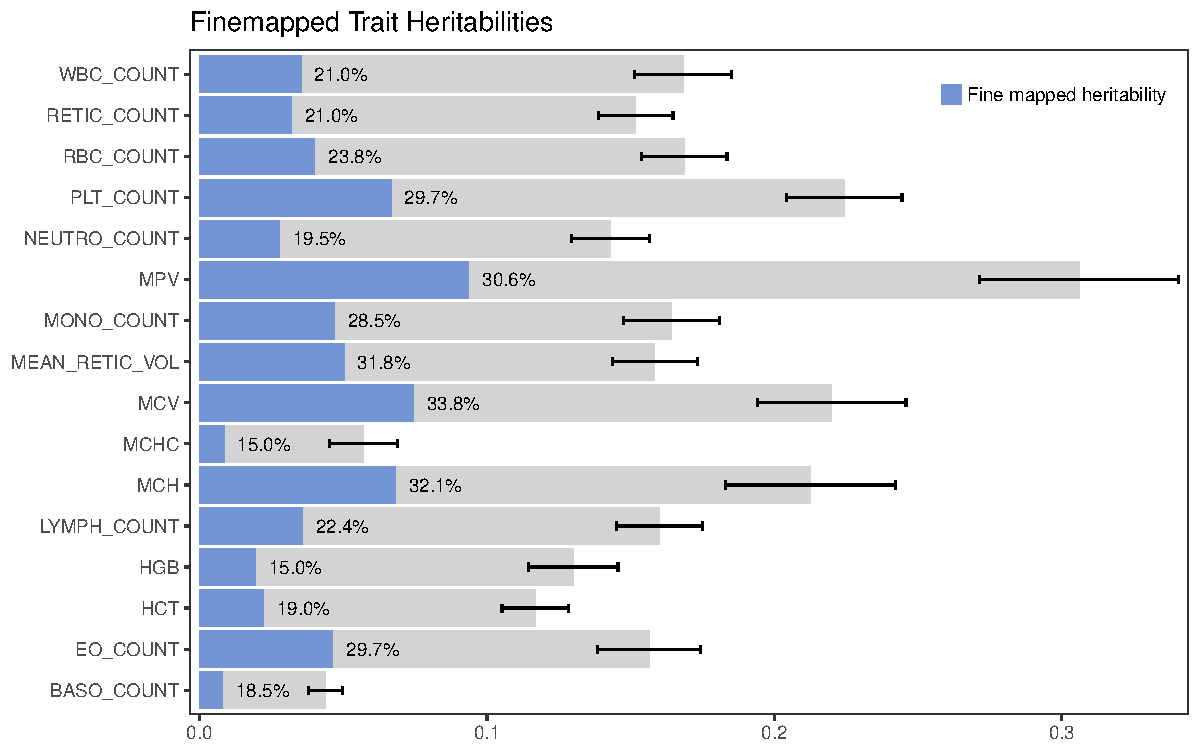
\includegraphics[width=\maxwidth]{figure/heritabilityPlots-1} 

}

\caption[Heritability estimates from LD Score Regression across 16 hematopoetic traits]{Heritability estimates from LD Score Regression across 16 hematopoetic traits. The estimates of the narrow-sense SNP heritabilities are plotted in gray with their corresponding standard erors. Heritability estimates for all variants with fine-mapped posterior probability > 0.001 are plotted in blue for each trait, and the proportions of total narrow-sense heritability captured by these fine-mapped variants (blue bar / gray bar) are indicated by the numbered labels.}\label{fig:heritabilityPlots}
\end{figure}


\end{knitrout}

\begin{knitrout}
\definecolor{shadecolor}{rgb}{0.969, 0.969, 0.969}\color{fgcolor}\begin{figure}[H]

{\centering 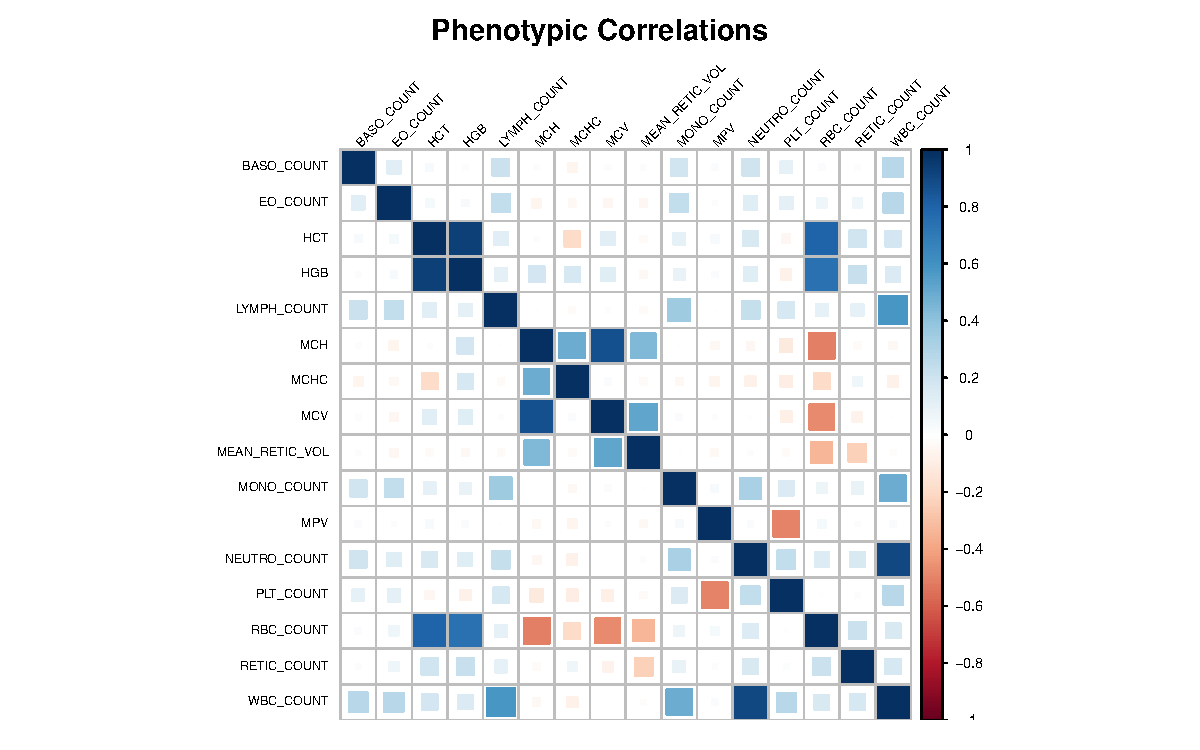
\includegraphics[width=\maxwidth]{figure/correlationPlots-1} 

}

\caption[Phenotypic and genetic correlations across the 16 traits examined]{Phenotypic and genetic correlations across the 16 traits examined. }\label{fig:correlationPlots}
\end{figure}


\end{knitrout}





\begin{knitrout}
\definecolor{shadecolor}{rgb}{0.969, 0.969, 0.969}\color{fgcolor}\begin{figure}[H]

{\centering 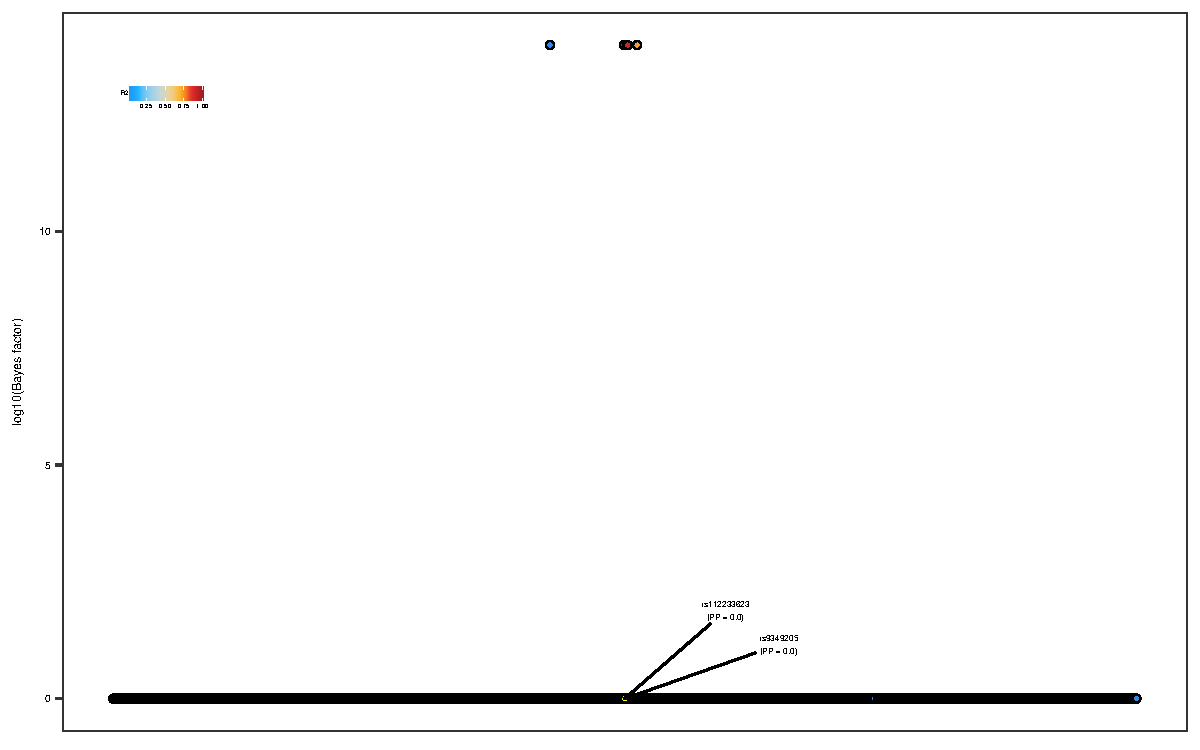
\includegraphics[width=\maxwidth]{figure/ccnd3UK10KLD-1} 

}

\caption[Fine-mapped log10(Bayes factor) values for CCND3 variants, with LD estimated from a reference panel of 3,677 individuals from the UK10K cohort]{Fine-mapped log10(Bayes factor) values for CCND3 variants, with LD estimated from a reference panel of 3,677 individuals from the UK10K cohort.}\label{fig:ccnd3UK10KLD}
\end{figure}


\end{knitrout}

\begin{knitrout}
\definecolor{shadecolor}{rgb}{0.969, 0.969, 0.969}\color{fgcolor}\begin{figure}[H]

{\centering 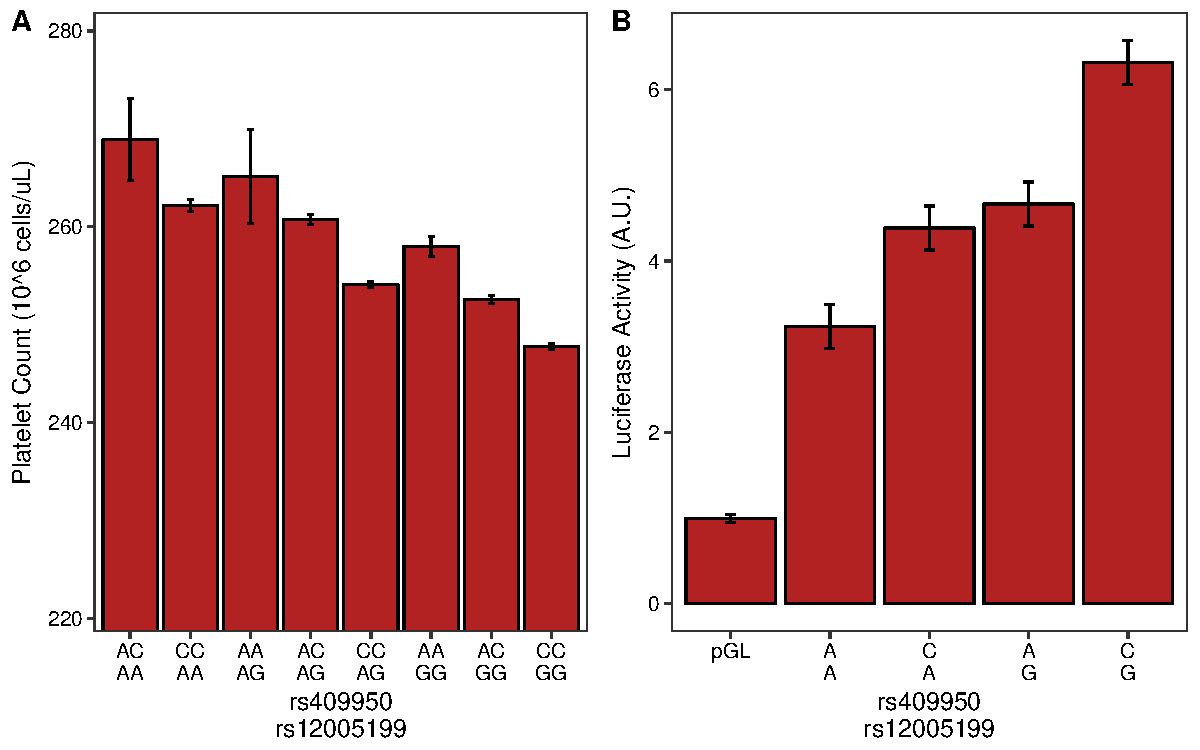
\includegraphics[width=\maxwidth]{figure/ak3Phenos/Reporter-1} 

}

\caption[Effects of AK3 variants rs409950 and rs12005199 on platelet count]{Effects of AK3 variants rs409950 and rs12005199 on platelet count. (A) rs409950/rs12005199 haplotypes exert additive effects on platelet count amongst individuals from the UKBB GWAS. (B) Luciferase reporter assay corroborates additive effects of the two SNPs on transcription.}\label{fig:ak3Phenos/Reporter}
\end{figure}


\end{knitrout}

\begin{figure}
\centering
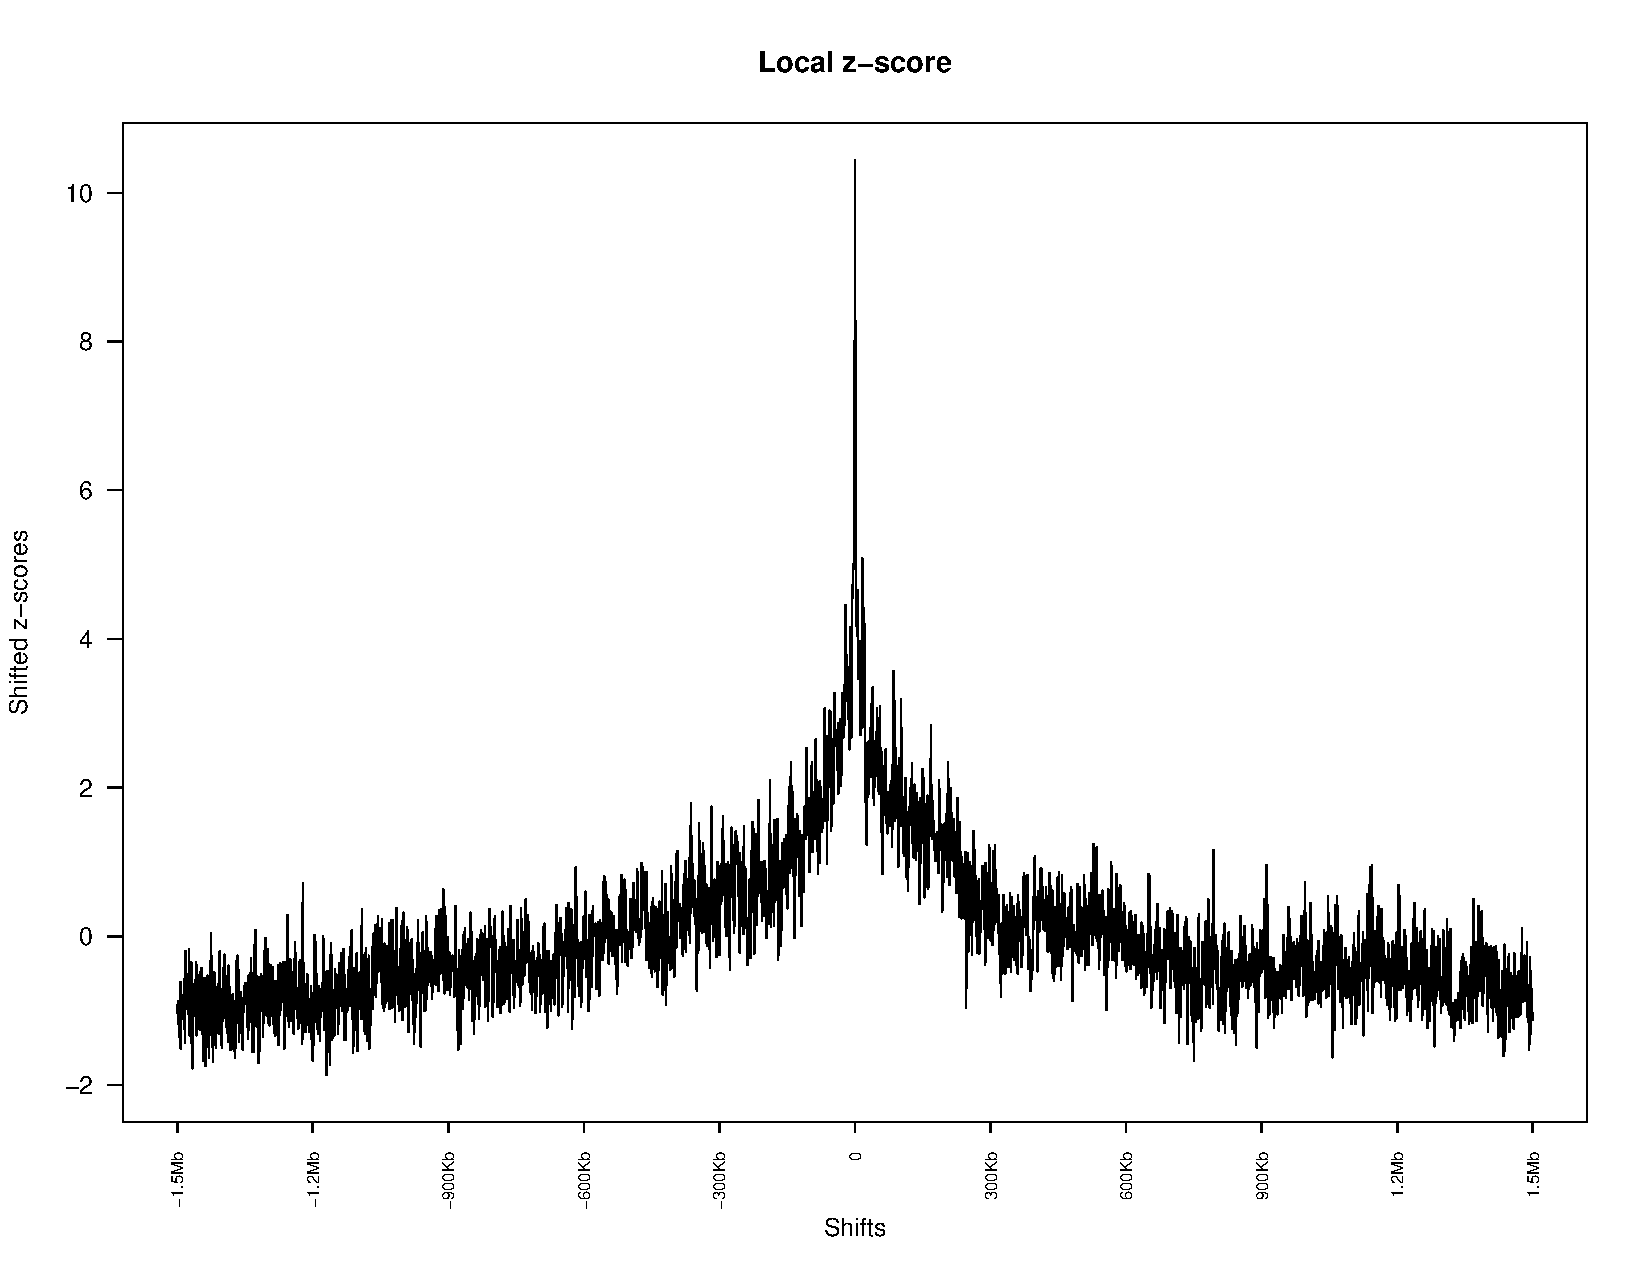
\includegraphics[width=\linewidth]{staticFigures/FINEMAP_PP10_localzscore_10000.pdf}
\caption{Local z-scores for enrichment of hematopoietic nucleosome-depleted regions in the set of fine-mapped variants with posterior probability $> 0.10$.}
\end{figure} 

\begin{figure}
\centering
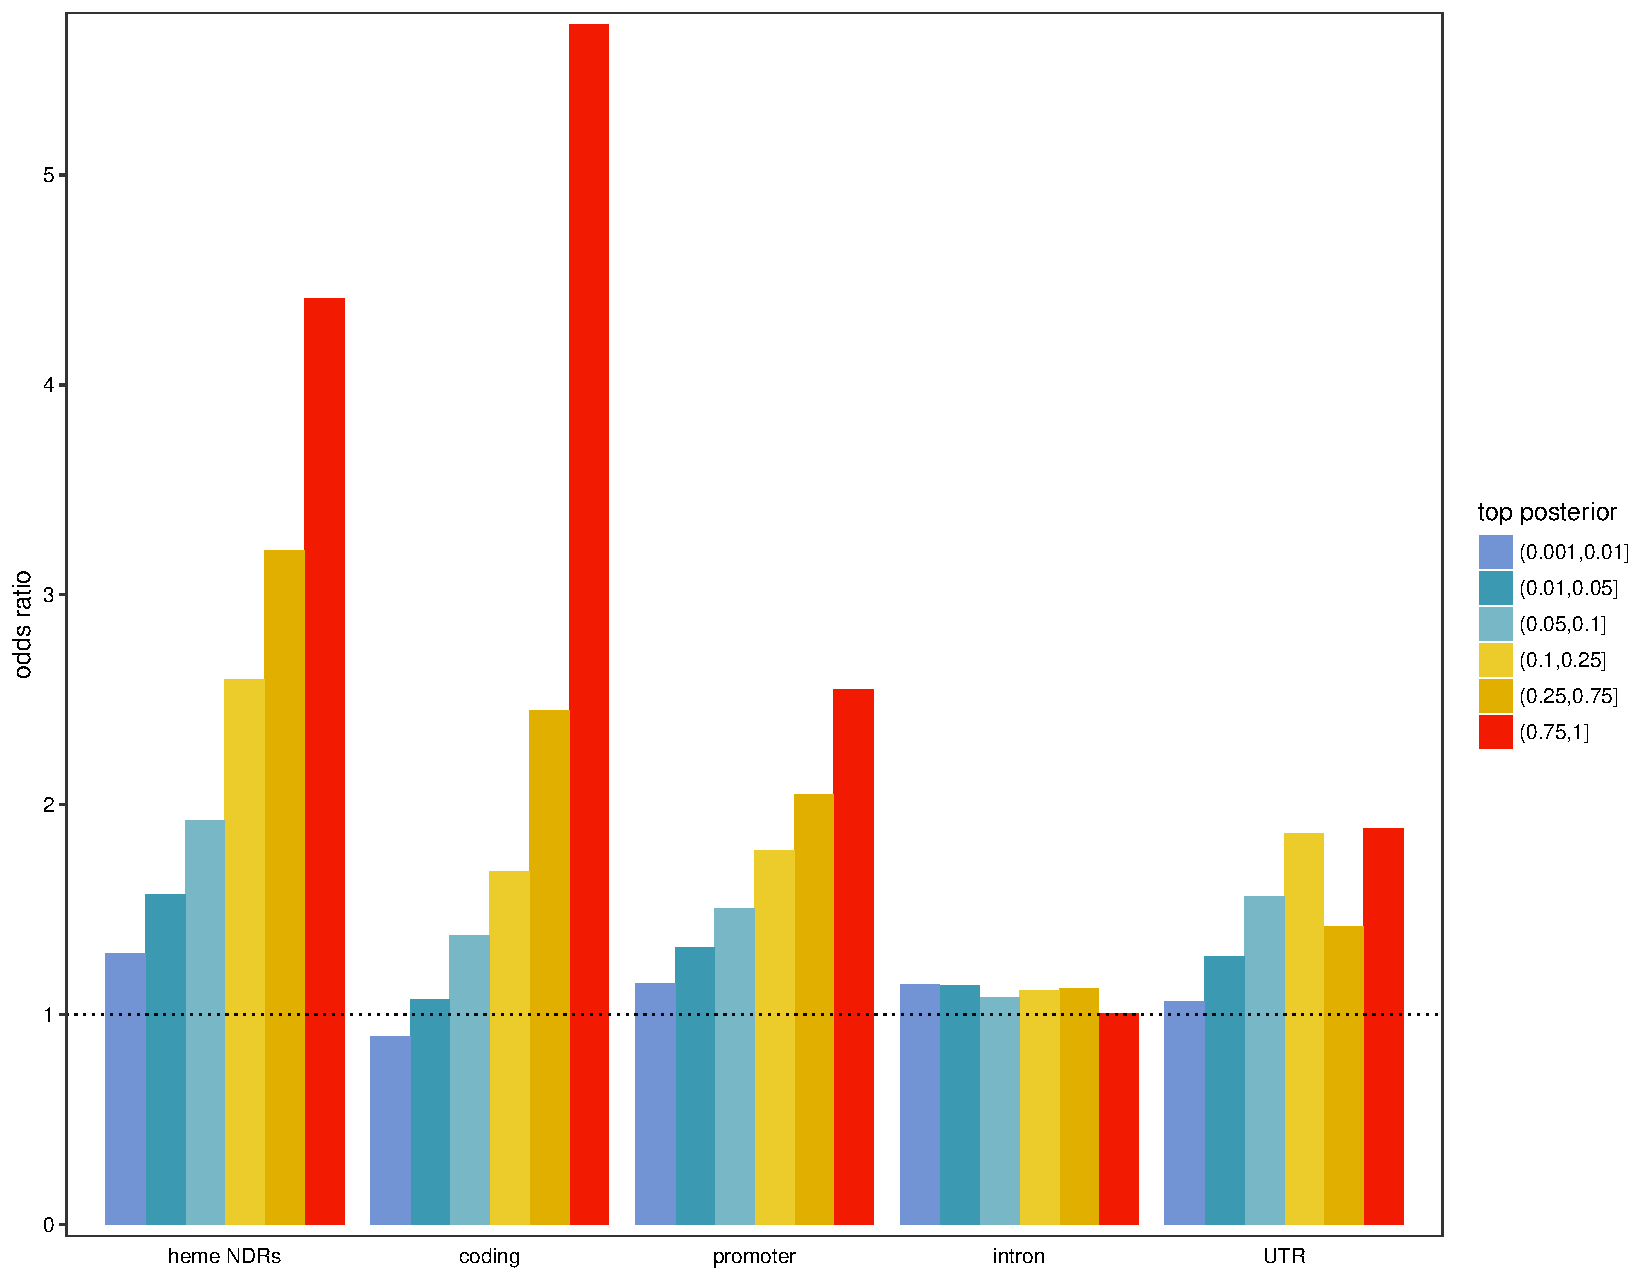
\includegraphics[width=\linewidth]{staticFigures/FINEMAP_enrichments_ExcludingSentinels.pdf}
\caption{Local annotation enrichments for fine-mapped variants, excluding all fine-map variants with $R^2>0.80$ to the sentinel variant of any region.}
\end{figure} 

\begin{figure}
\centering
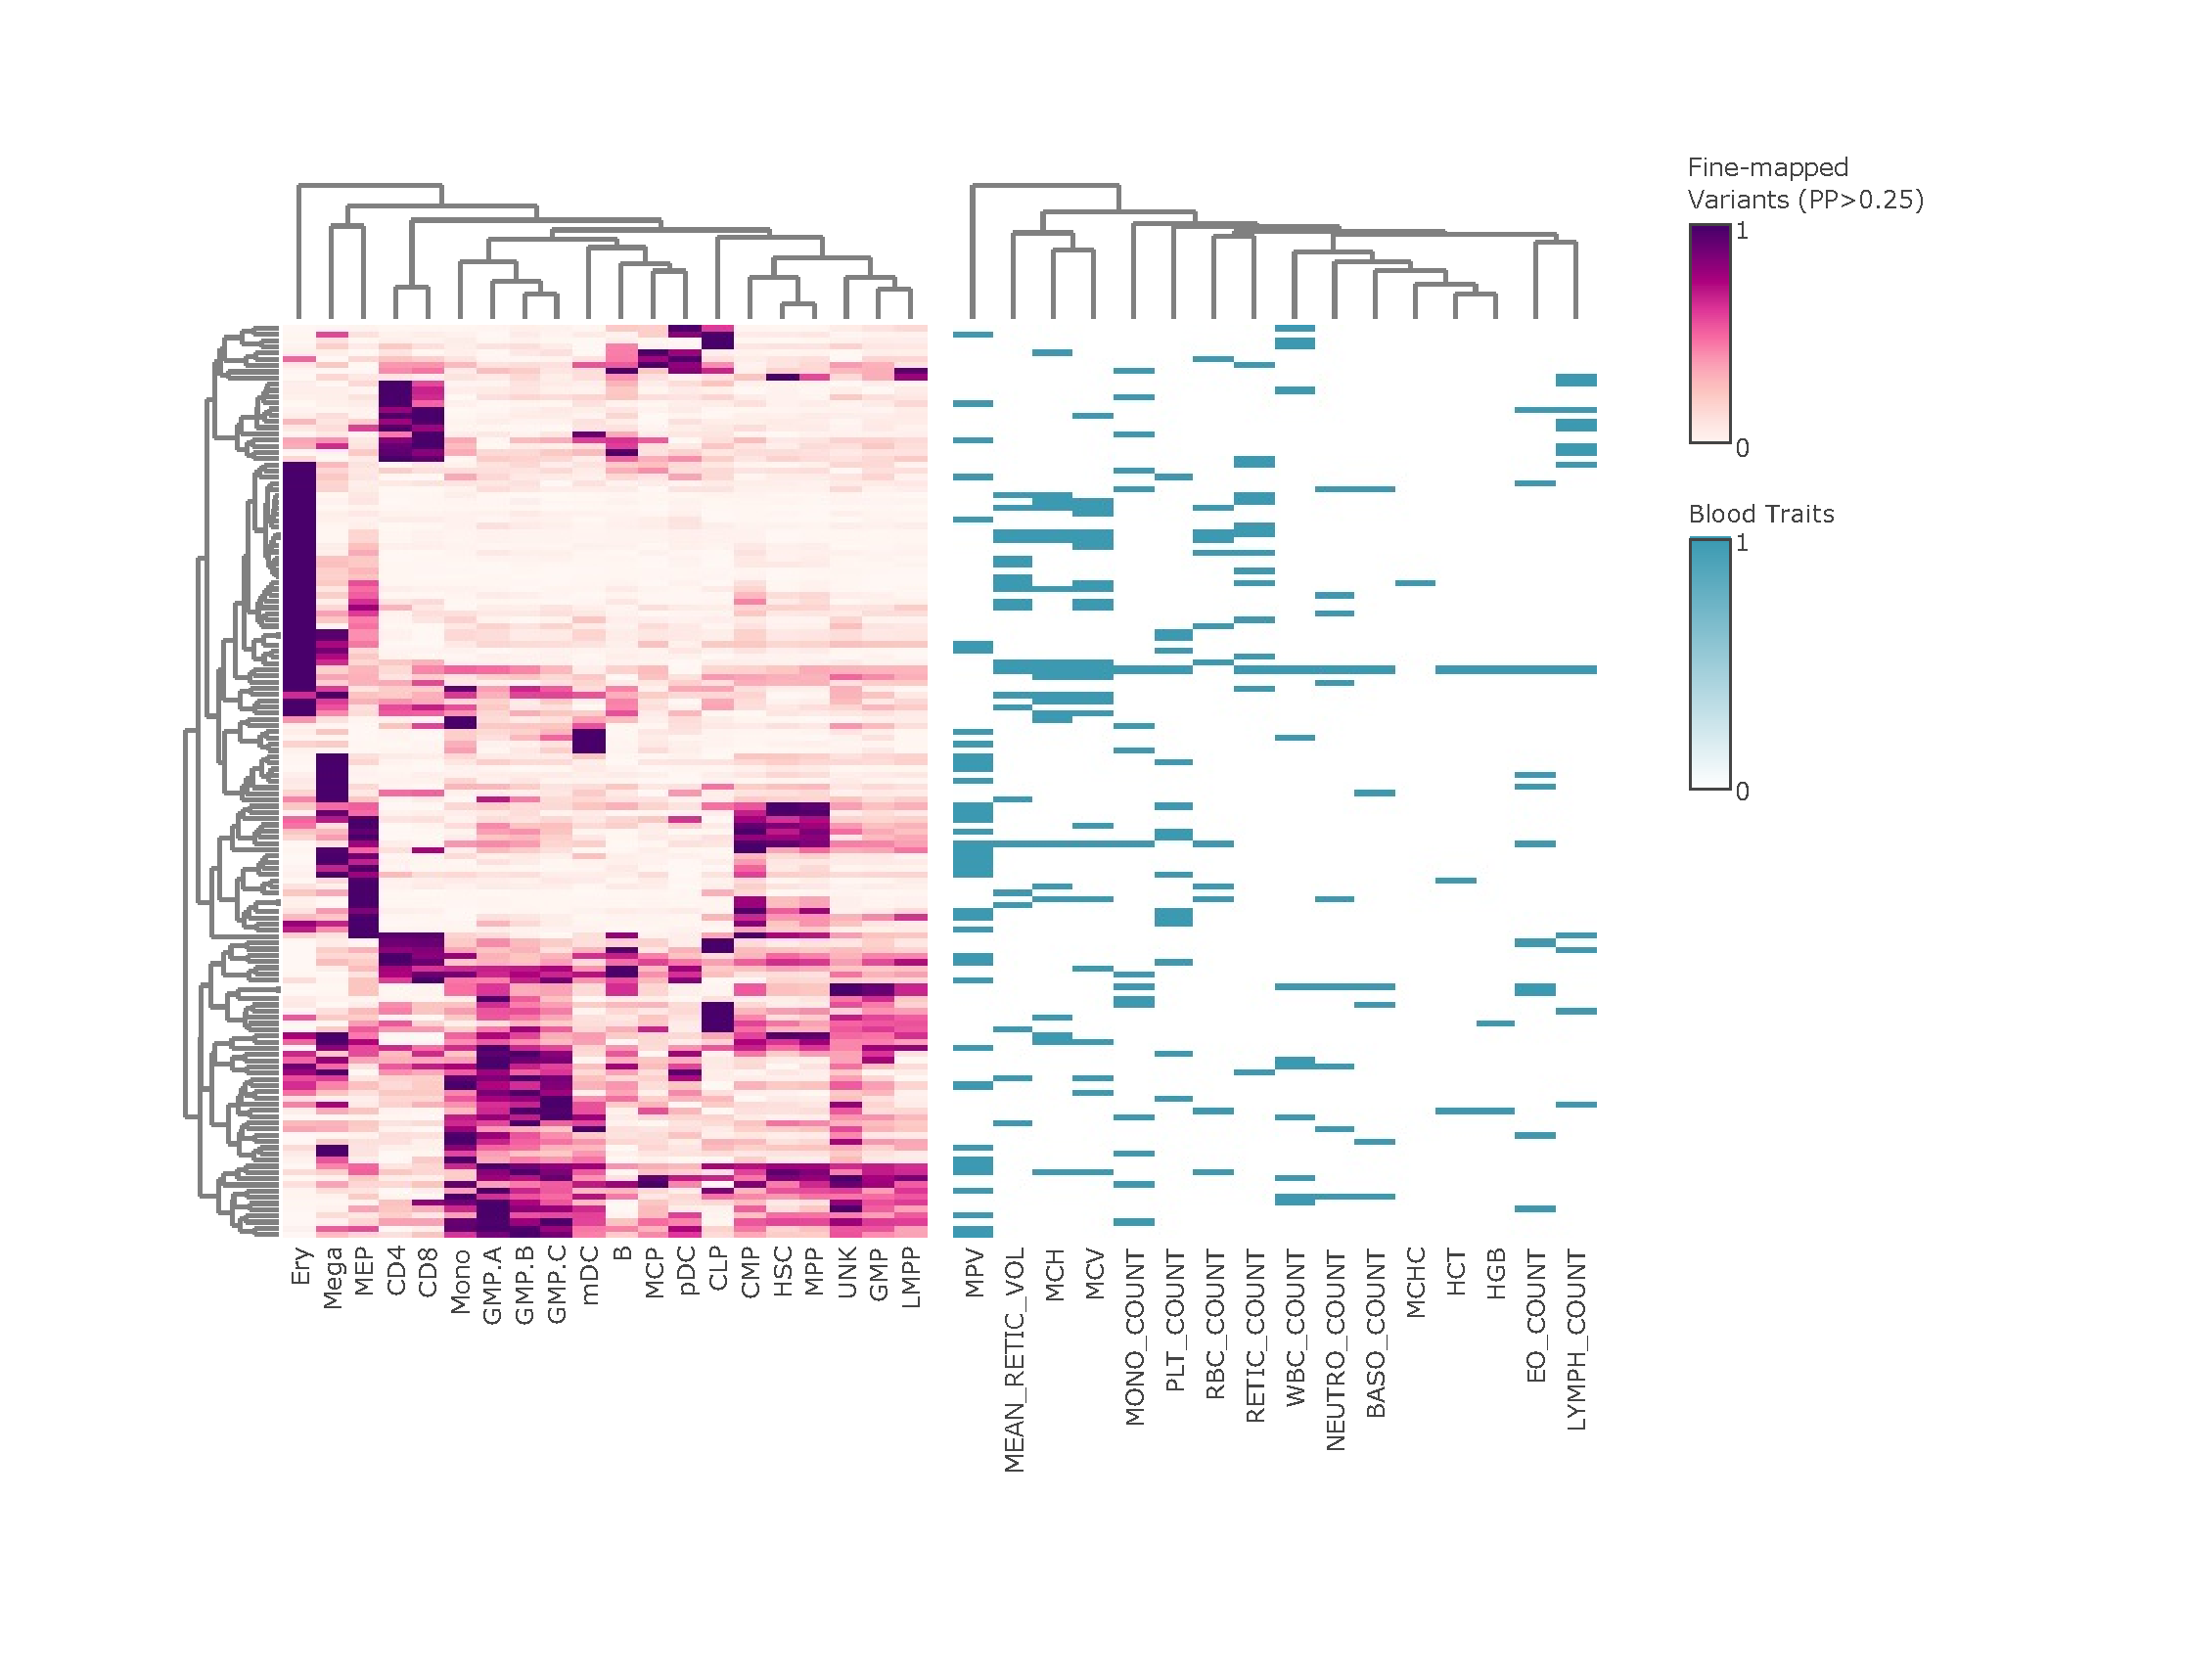
\includegraphics[width=\linewidth]{staticFigures/UKBB_PP50_bulk.pdf}
\caption{Side-by-side heatmaps showing overlap of hematopoietic nucleosome-depleted regions by cell type with fine-mapped variants ($PP>0.50$) by trait. The two heatmaps share a common y-axis of specific variants.}
\end{figure} 

\begin{knitrout}
\definecolor{shadecolor}{rgb}{0.969, 0.969, 0.969}\color{fgcolor}\begin{figure}[H]

{\centering 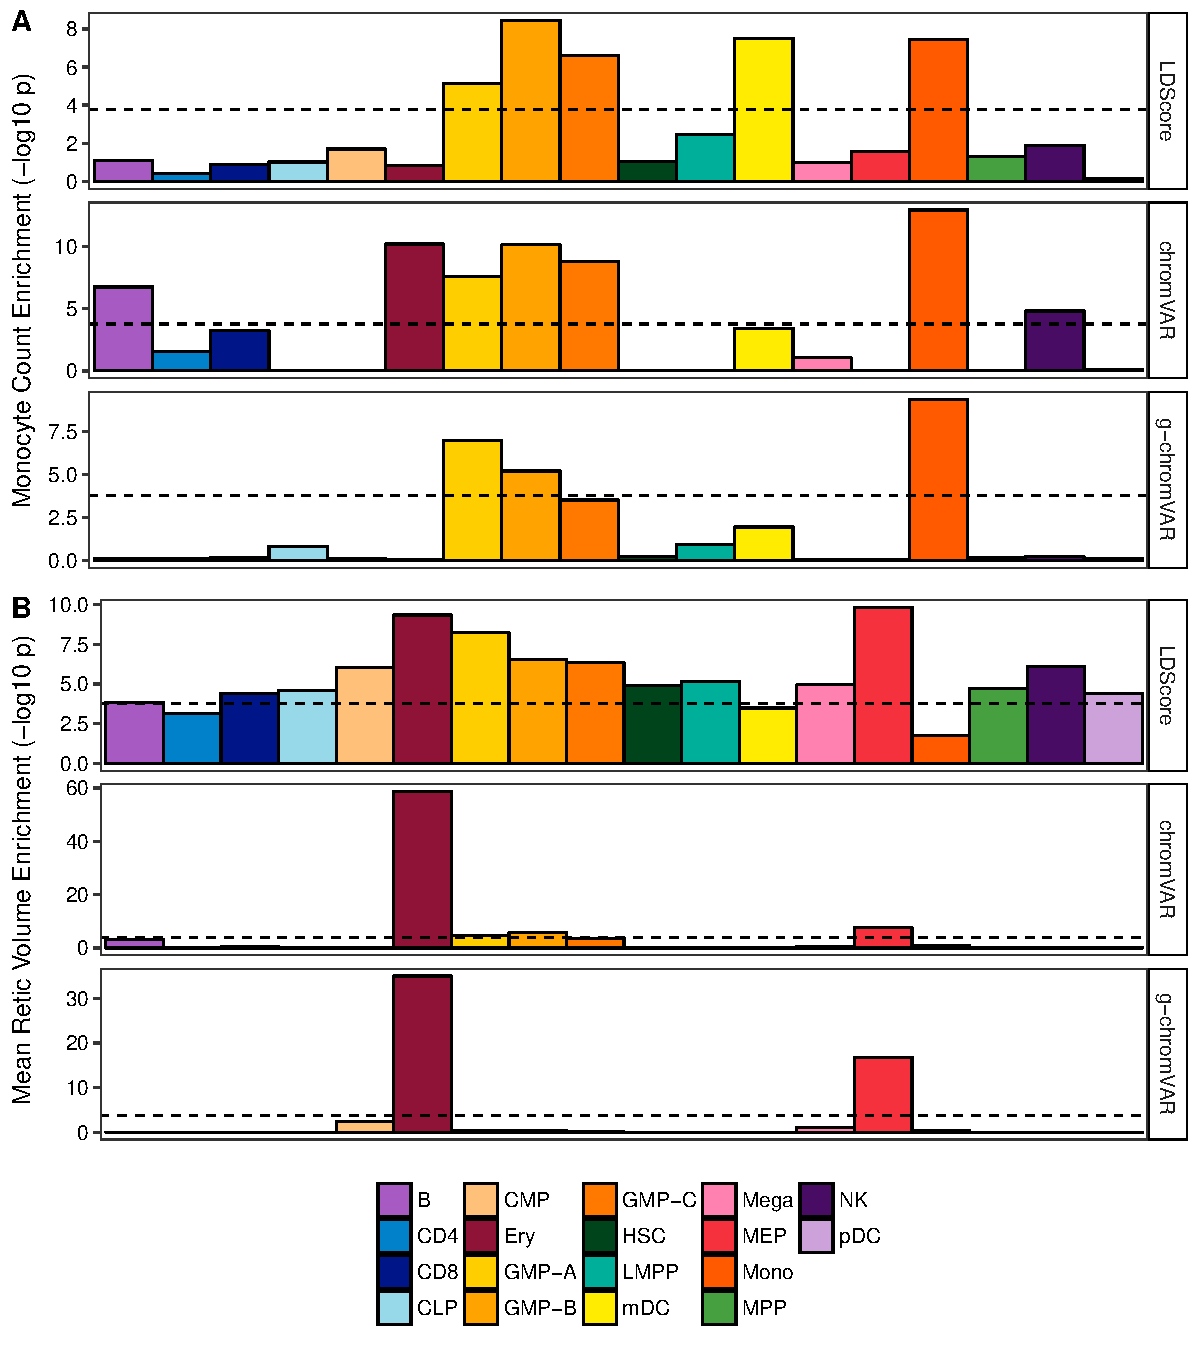
\includegraphics[width=\maxwidth]{figure/barplots-1} 

}

\caption[Hematopoetic cell type enrichments for Mean Retic Volume and Monocyte count using various methods]{Hematopoetic cell type enrichments for Mean Retic Volume and Monocyte count using various methods.}\label{fig:barplots}
\end{figure}


\end{knitrout}


\begin{knitrout}
\definecolor{shadecolor}{rgb}{0.969, 0.969, 0.969}\color{fgcolor}\begin{figure}[H]

{\centering 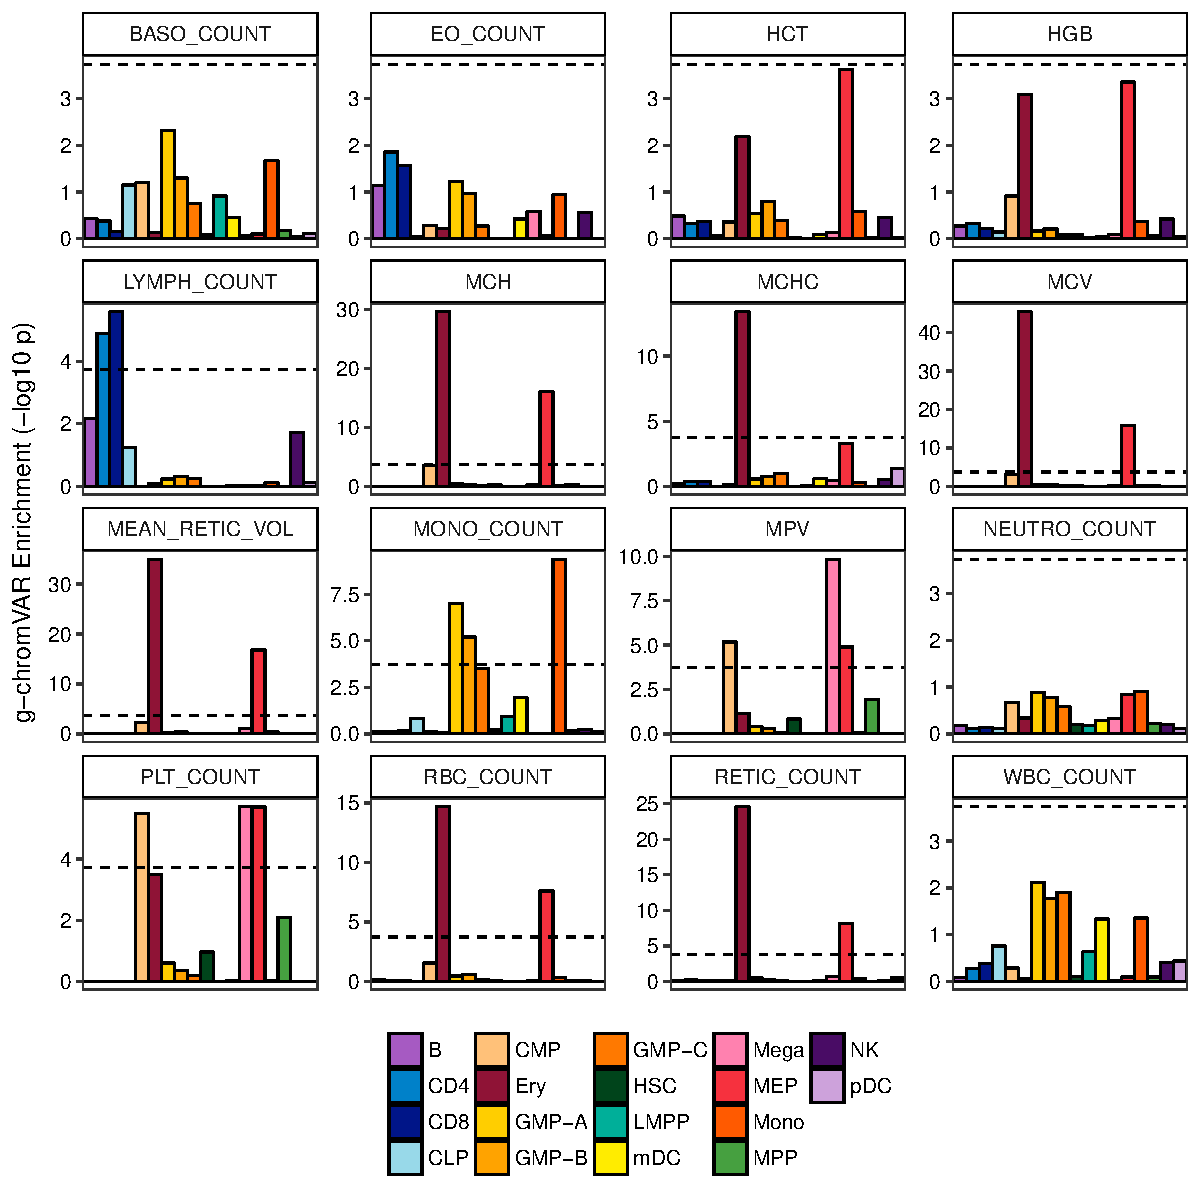
\includegraphics[width=\maxwidth]{figure/allGchromvar-1} 

}

\caption[All enrichments from g-chromVAR]{All enrichments from g-chromVAR. The horizontal line shows a Bonferonni multiple testing adjusted threshold for statistical significance of enrichment.}\label{fig:allGchromvar}
\end{figure}


\end{knitrout}

\begin{knitrout}
\definecolor{shadecolor}{rgb}{0.969, 0.969, 0.969}\color{fgcolor}\begin{figure}[H]

{\centering 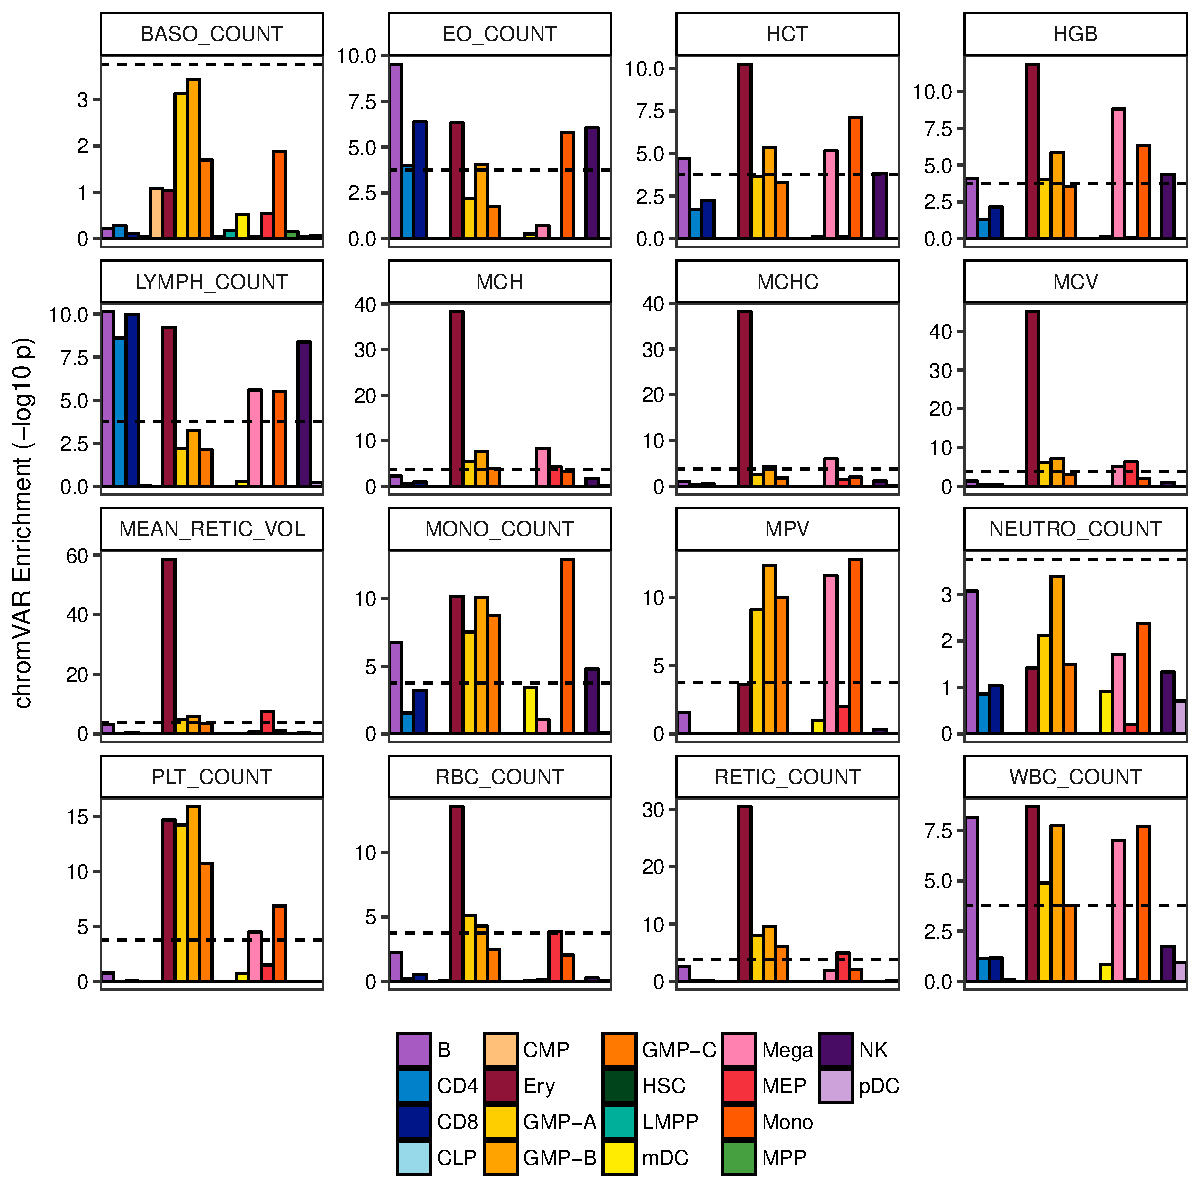
\includegraphics[width=\maxwidth]{figure/allchromVAR-1} 

}

\caption[All enrichments from chromVAR]{All enrichments from chromVAR. The horizontal line shows a Bonferonni multiple testing adjusted threshold for statistical significance of enrichment.}\label{fig:allchromVAR}
\end{figure}


\end{knitrout}

\begin{knitrout}
\definecolor{shadecolor}{rgb}{0.969, 0.969, 0.969}\color{fgcolor}\begin{figure}[H]

{\centering 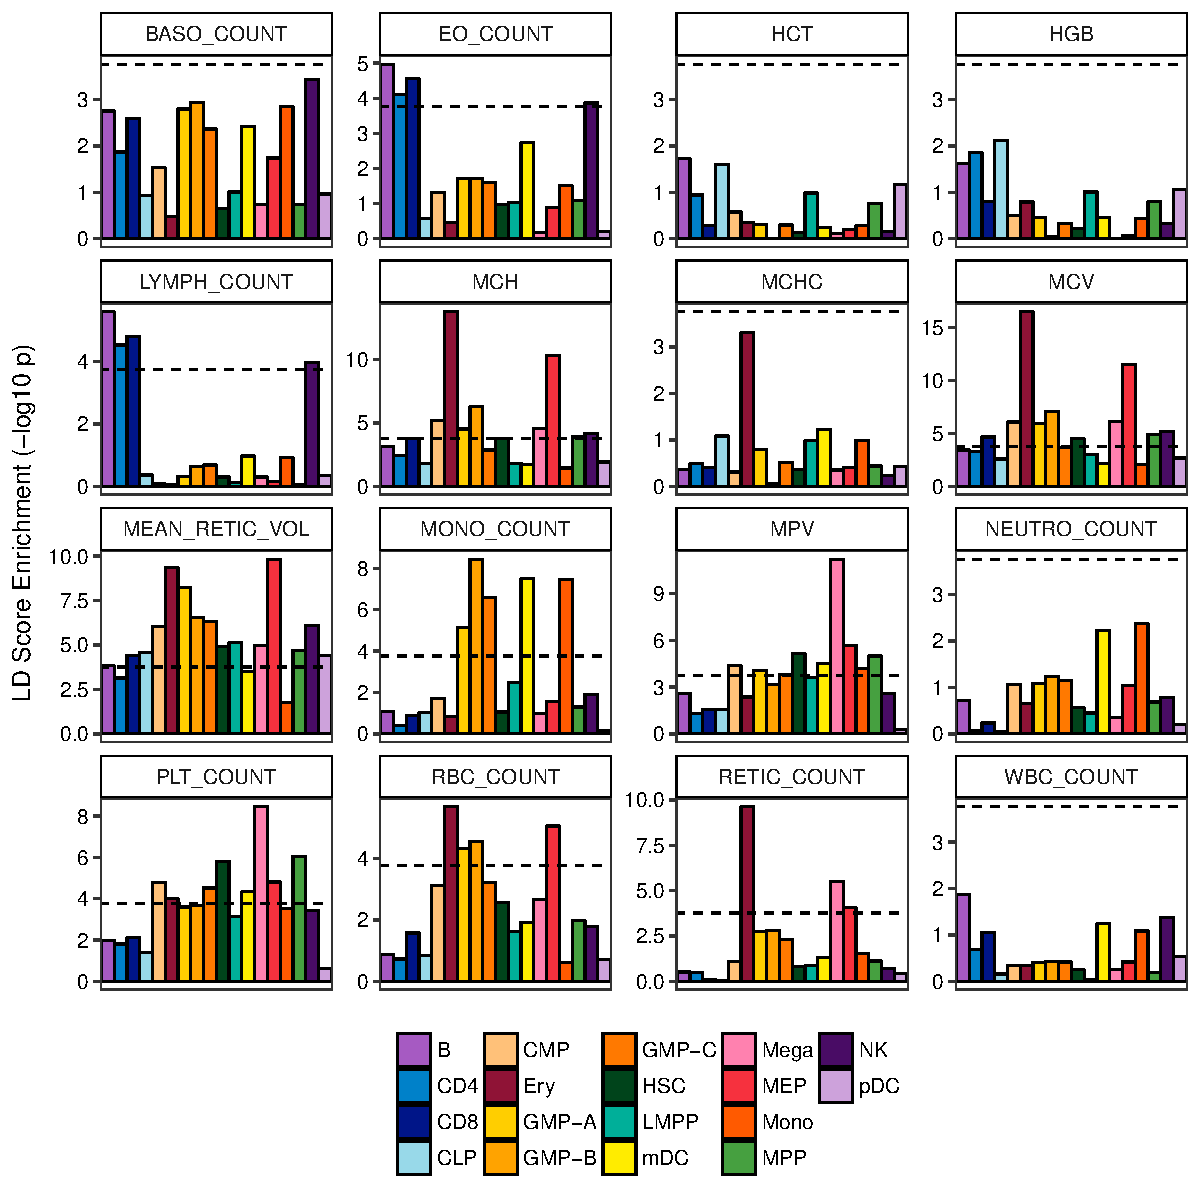
\includegraphics[width=\maxwidth]{figure/allLDscore-1} 

}

\caption[All enrichments from LD score regression, calculated from the z-scores of the coefficients for each cell-type-specific annotation added separately to the baseline model]{All enrichments from LD score regression, calculated from the z-scores of the coefficients for each cell-type-specific annotation added separately to the baseline model. The horizontal line shows a Bonferonni multiple testing adjusted threshold for statistical significance of enrichment.}\label{fig:allLDscore}
\end{figure}


\end{knitrout}

\begin{knitrout}
\definecolor{shadecolor}{rgb}{0.969, 0.969, 0.969}\color{fgcolor}\begin{figure}[H]

{\centering 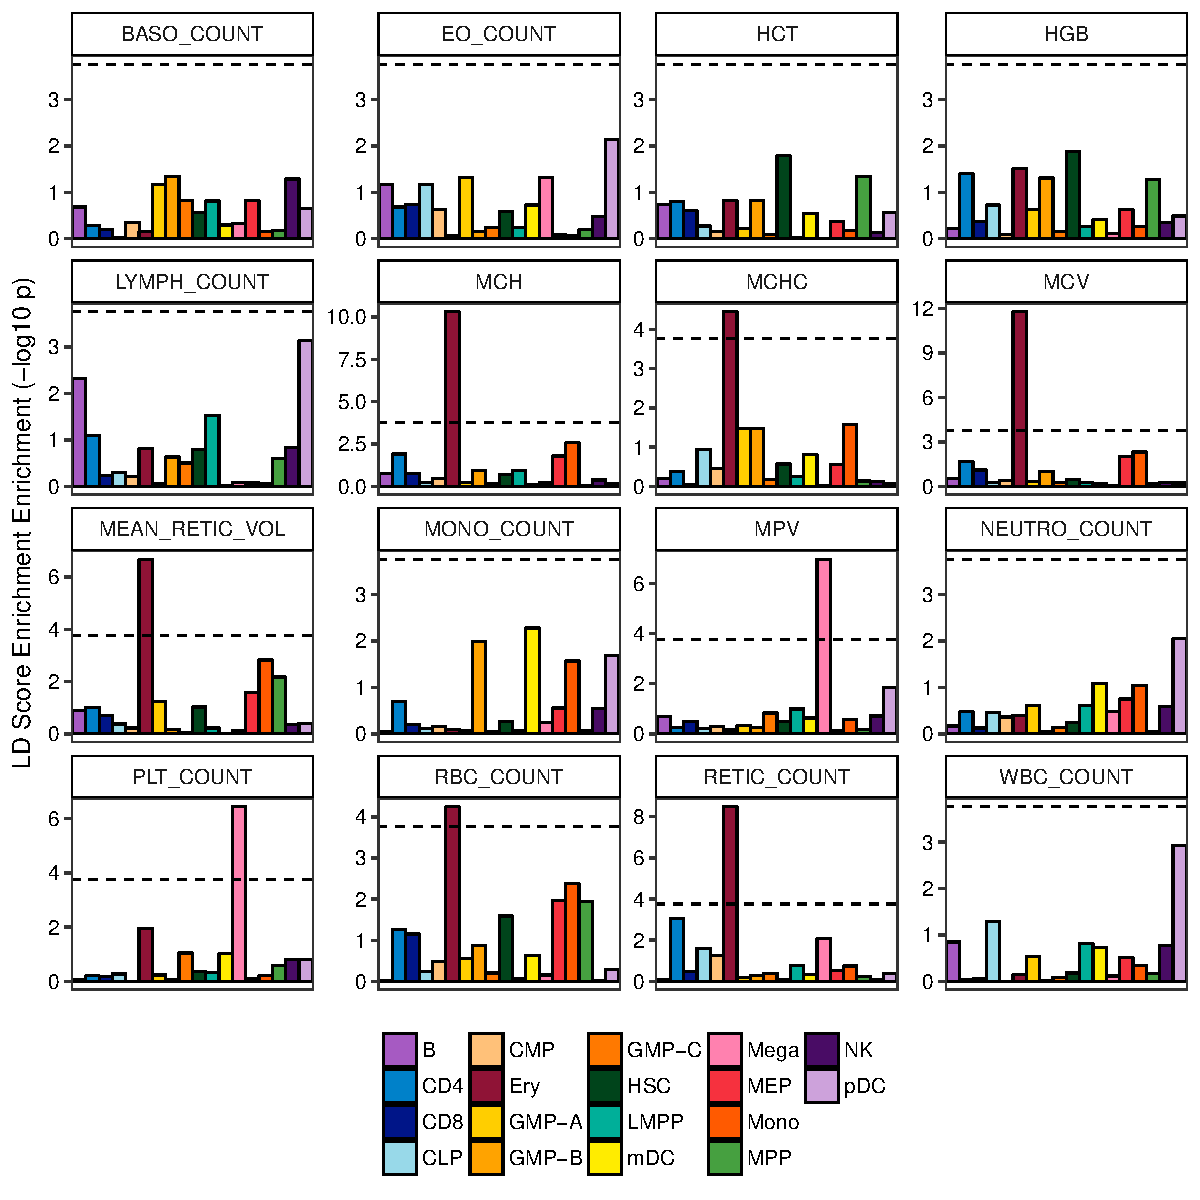
\includegraphics[width=\maxwidth]{figure/panhemeLDscore-1} 

}

\caption[All enrichments from LD score regression, calculated from coefficient z-scores after jointly adding all 18 cell-type-specific annotations to the baseline model at once]{All enrichments from LD score regression, calculated from coefficient z-scores after jointly adding all 18 cell-type-specific annotations to the baseline model at once. The horizontal line shows a Bonferonni multiple testing adjusted threshold for statistical significance of enrichment.}\label{fig:panhemeLDscore}
\end{figure}


\end{knitrout}

\begin{knitrout}
\definecolor{shadecolor}{rgb}{0.969, 0.969, 0.969}\color{fgcolor}\begin{figure}[H]

{\centering 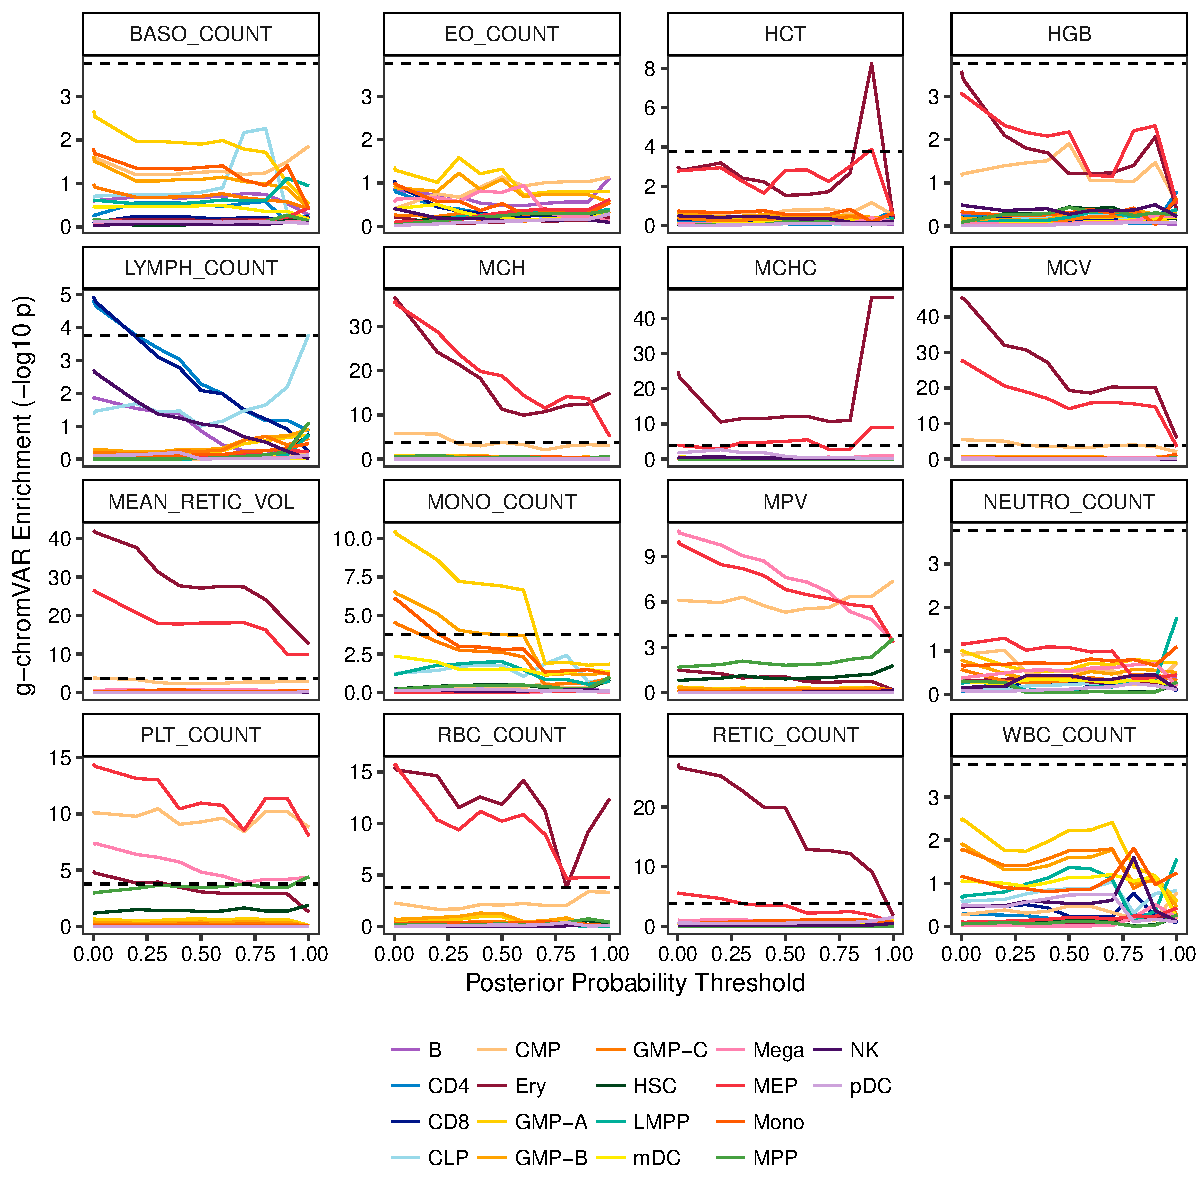
\includegraphics[width=\maxwidth]{figure/varyingPP-1} 

}

\caption[Cell type - trait enrichments for g-chromVAR across different finemap variants posterior probability cutoffs]{Cell type - trait enrichments for g-chromVAR across different finemap variants posterior probability cutoffs. The horizontal line shows a Bonferonni multiple testing adjusted threshold for statistical significance of enrichment.}\label{fig:varyingPP}
\end{figure}


\end{knitrout}





\begin{knitrout}
\definecolor{shadecolor}{rgb}{0.969, 0.969, 0.969}\color{fgcolor}\begin{figure}[H]

{\centering 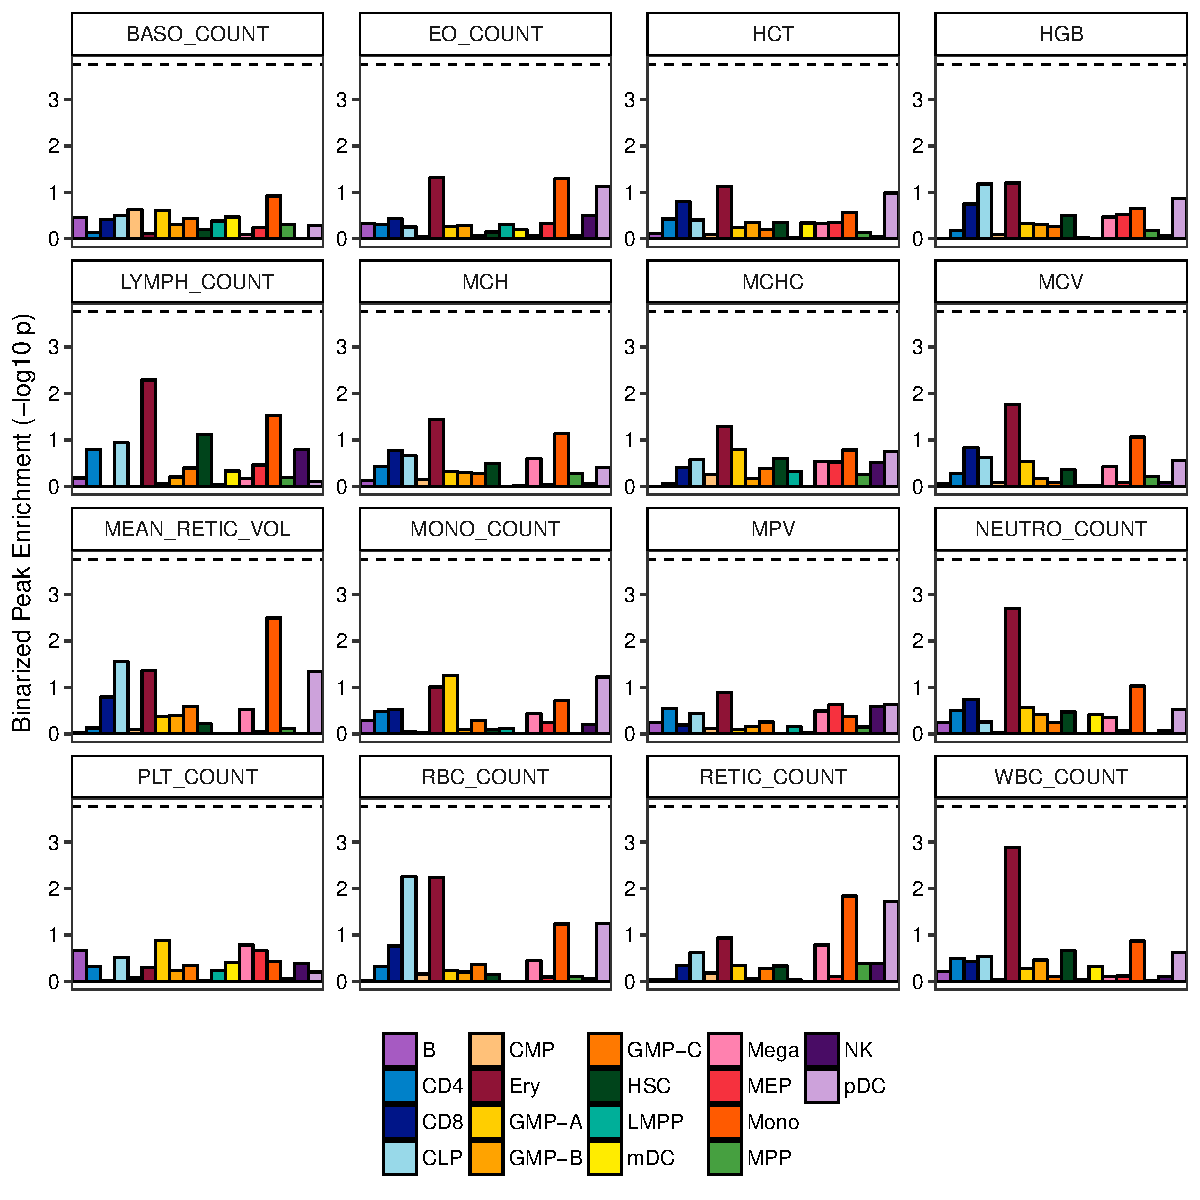
\includegraphics[width=\maxwidth]{figure/binarizedPeakPlot-1} 

}

\caption[Results of trait/cell type enrichments across hematopoesis using binarized peaks]{Results of trait/cell type enrichments across hematopoesis using binarized peaks. These results demonstrate the importance of accounting for quantitative chromatin values in peaks to be powered for detecting enriched cell types and traits.}\label{fig:binarizedPeakPlot}
\end{figure}


\end{knitrout}

\begin{knitrout}
\definecolor{shadecolor}{rgb}{0.969, 0.969, 0.969}\color{fgcolor}\begin{figure}[H]

{\centering 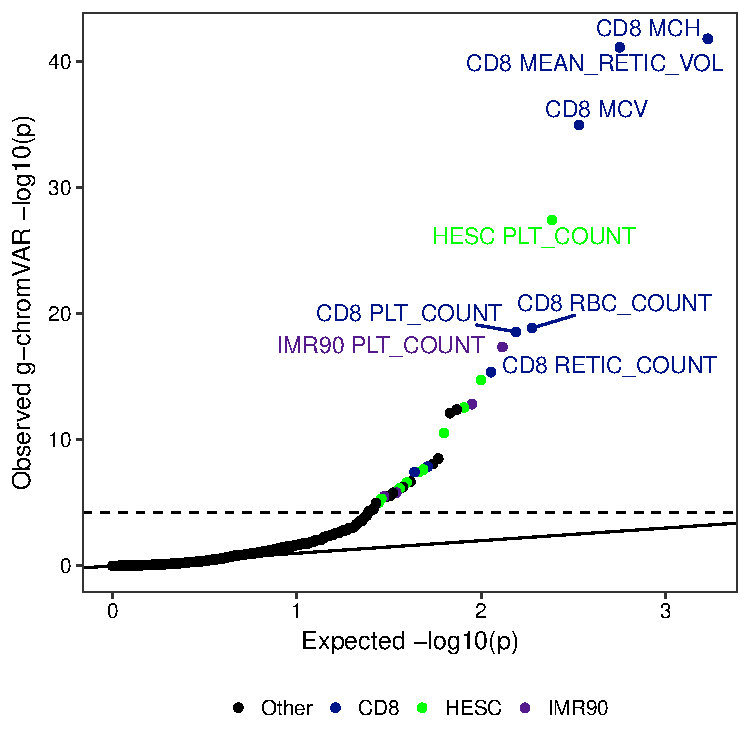
\includegraphics[width=\maxwidth]{figure/roadmapPlot-1} 

}

\caption[QQplot of observed and expected enrichments using DNase hypersensitivity data and identical pre-processing for 53 tissue types from Roadmap]{QQplot of observed and expected enrichments using DNase hypersensitivity data and identical pre-processing for 53 tissue types from Roadmap. The top eight pairs of cell types and traits are annotated on the plot where 35 total pairs passed Bonferroni-adjusted significance. }\label{fig:roadmapPlot}
\end{figure}


\end{knitrout}

\begin{knitrout}
\definecolor{shadecolor}{rgb}{0.969, 0.969, 0.969}\color{fgcolor}\begin{figure}[H]

{\centering 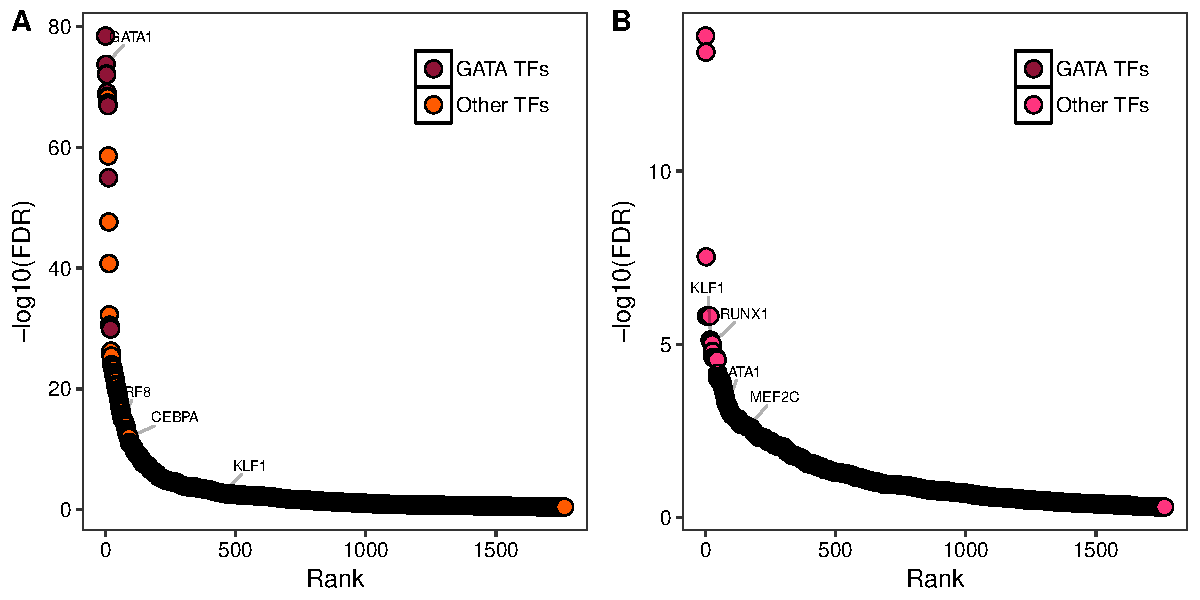
\includegraphics[width=\maxwidth]{figure/tfRankOrderPlots-1} 

}

\caption[Two subpopulations of CMP and MEP cells were obtained by k-medoids clustering on ATAC principal components or g-ChromVAR enrichments, respectively]{Two subpopulations of CMP and MEP cells were obtained by k-medoids clustering on ATAC principal components or g-ChromVAR enrichments, respectively. Rank-order plots showing transcription factor binding sites ranked by difference in chromVAR enrichment between the two clusters of (A) CMP and (B) MEP populations}\label{fig:tfRankOrderPlots}
\end{figure}


\end{knitrout}

\end{document}
